\documentclass[12pt,a4paper]{article}
\usepackage[utf8]{inputenc}
\usepackage{graphicx}
\usepackage{tikz}
\usetikzlibrary{fit}
\usepackage{lmodern}
\usepackage{sectsty}
\usepackage{float}
\usepackage{titlesec}
\usepackage{listings}
\usepackage{color}
\usepackage[hyphens]{url}
\usepackage{hyperref}

\hypersetup{  
	colorlinks=true,
    linkcolor=black,
    filecolor=magenta,      
    urlcolor=cyan,
}

\definecolor{dkgreen}{rgb}{0,0.6,0}
\definecolor{gray}{rgb}{0.5,0.5,0.5}
\definecolor{mauve}{rgb}{0.58,0,0.82}

\lstset{frame=tb,
  language=sh,
  aboveskip=3mm,
  belowskip=3mm,
  showstringspaces=false,
  columns=flexible,
  basicstyle={\small\ttfamily},
  numbers=none,
  numberstyle=\tiny\color{gray},
  keywordstyle=\color{blue},
  commentstyle=\color{dkgreen},
  stringstyle=\color{mauve},
  breaklines=true,
  breakatwhitespace=true,
  tabsize=3
}

\setcounter{secnumdepth}{4}

\titleformat{\paragraph}
{\normalfont\normalsize\bfseries}{\theparagraph}{1em}{}
\titlespacing*{\paragraph}
{0pt}{3.25ex plus 1ex minus .2ex}{1.5ex plus .2ex}
\sectionfont{\color{cyan}}

\begin{document}
   \begin{titlepage}
      {\fontfamily{lmss}\selectfont
      	\centering
      	
\includegraphics[width=0.30\textwidth]{logo.png}\par\vspace{1cm}
      	{\LARGE SplitBill Application \par}
      	\vspace{0.25cm}
      	{\huge\bfseries \color{cyan}User Manual\par}
      	\vspace{1cm}
      	{\Large\textit{by} Brute Force for Compiax\par}
         \vspace{0.25cm}
         \begin{tikzpicture}
            \node [inner sep=0pt,,outer sep=0pt,clip,rounded corners=0.5cm] (pict) at (0,0) {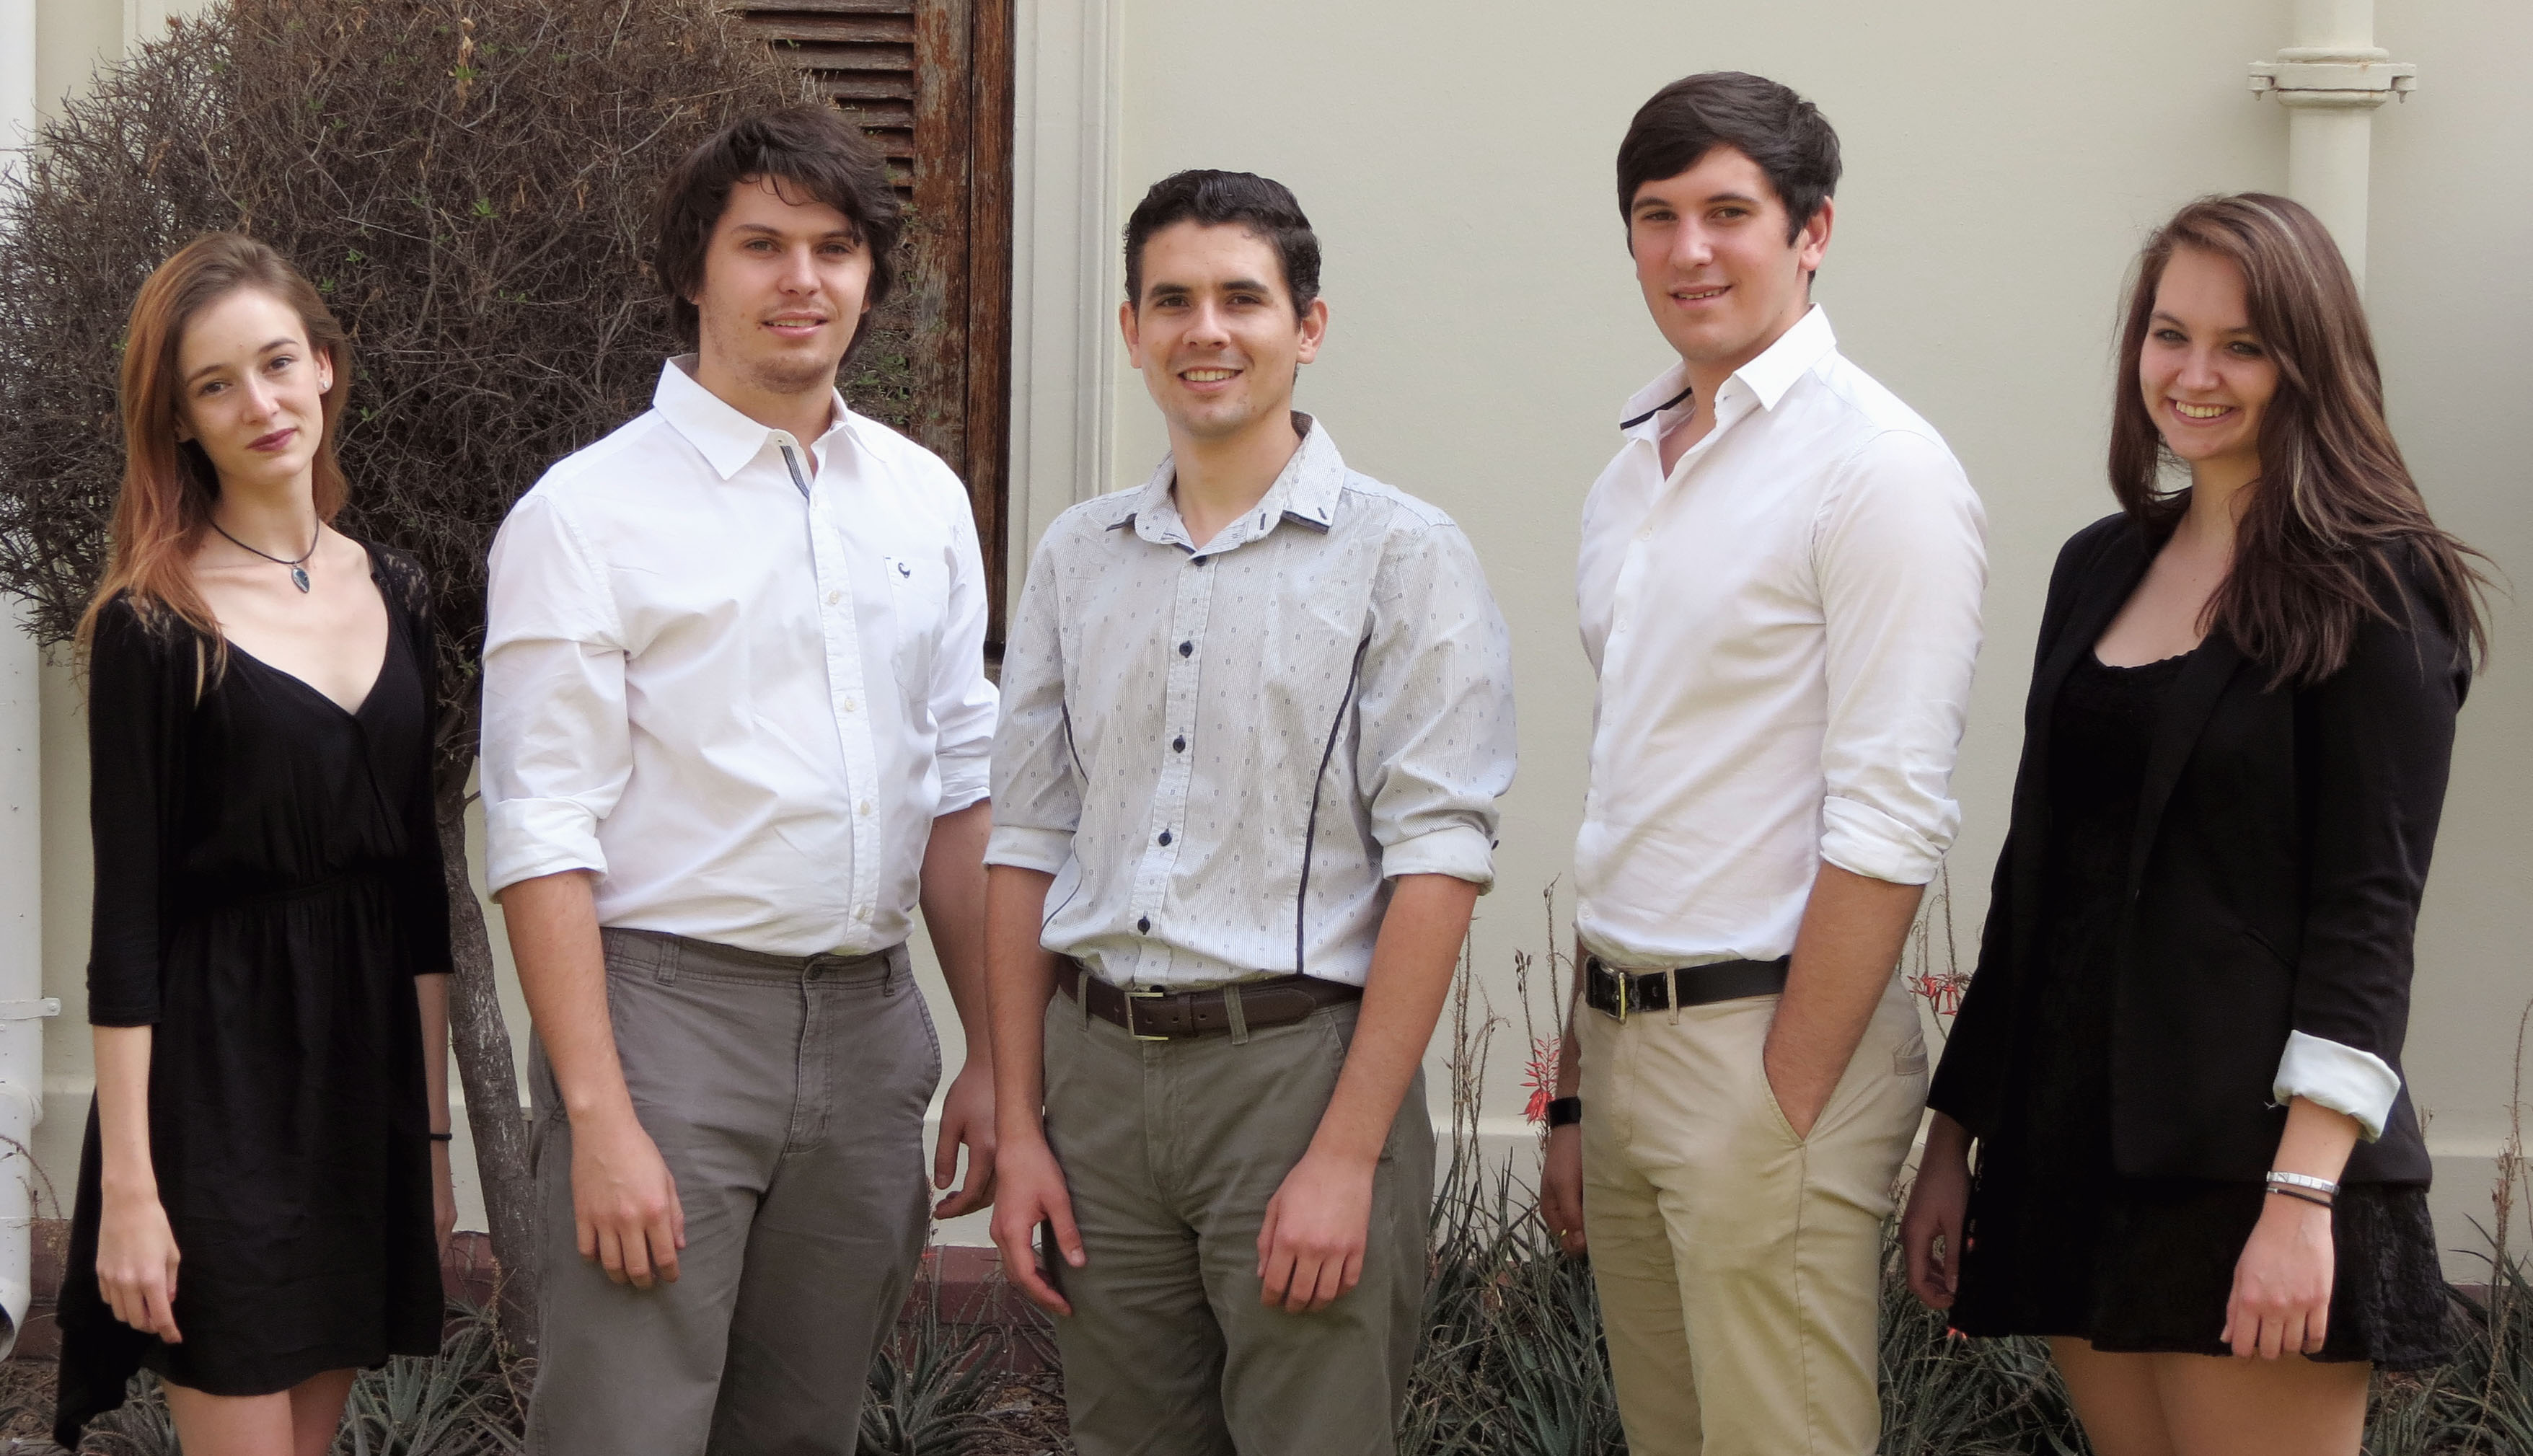
\includegraphics[width=0.9\textwidth]{team.jpg}};
            \node[fit=(pict),rounded corners=.55cm,inner sep=2pt]{};
         \end{tikzpicture}

         \par\vspace{1cm}
         \date{}
         \author{}
         \title{}
         \centering
         \textbf{Authors:}\\
         Mia Gerber\\
         Matthew Perry\\
         Wanrick Willemse\\
         Duart Breedt\\
         Linda Potgieter\\
      }
   \end{titlepage}
   \maketitle
   \tableofcontents
   \newpage
   
\section{General Information}
	\subsection{System Overview}
   The SplitBill application was made to facilitate the splitting of expenses based on a receipt image. The application uses optical character recognition technology to read item details from a bill. These details are displayed to the users on their devices and enable users to claim items from the bill. Claiming an item adds the item price to a displayed total which is the total amount that the user owes on the bill based on the items claimed. When an item is claimed, the user has the option to claim multiple instances of these items, and the user can also remove the items they have claimed if an error was made.  
     \subparagraph{}
     With this application, a large group of friends, co-workers or family members can easily calculate how much each person must pay for their own bill items.  
   Multiple users can be added to one bill by entering the code generated for the session when the bill is uploaded for display. This allows different users to claim items on the same bill. When one user claims an item, the changes in quantities are propagated to all devices of currently active users. The application also has a built-in functionality that calculates the user's gratuity based on the calculated total. 
   \subparagraph{}
   In addition to claiming items, the users are also presented with different functionalities to modify the currently displayed bill. The users have the options to add items or edit the currently displayed items. These changes are displayed on all devices currently viewing the bill. 
   
    \subsection{System Configuration} 
   The server contains three docker containers. These three are independent and run the API, MongoDB database and OCR Python module respectively. Communication between the MongoDB database or OCR module and the API is done through POST requests between modules.
   
   \subparagraph{} The mobile application, which can be installed on any individual’s phone, communicates with the API on the server using POST requests over a network connection. Currently, the application is being built for debugging on individual devices. Once SplitBill meets all user satisfaction criteria, it will be released on the Android store for public use. Currently, it is developed to run on \emph{Android KitKat (4.4)} or newer; however, SplitBill is envisioned and has the potential to be released on additional platforms such as Apple IOS. 
 
\begin{figure}[h]
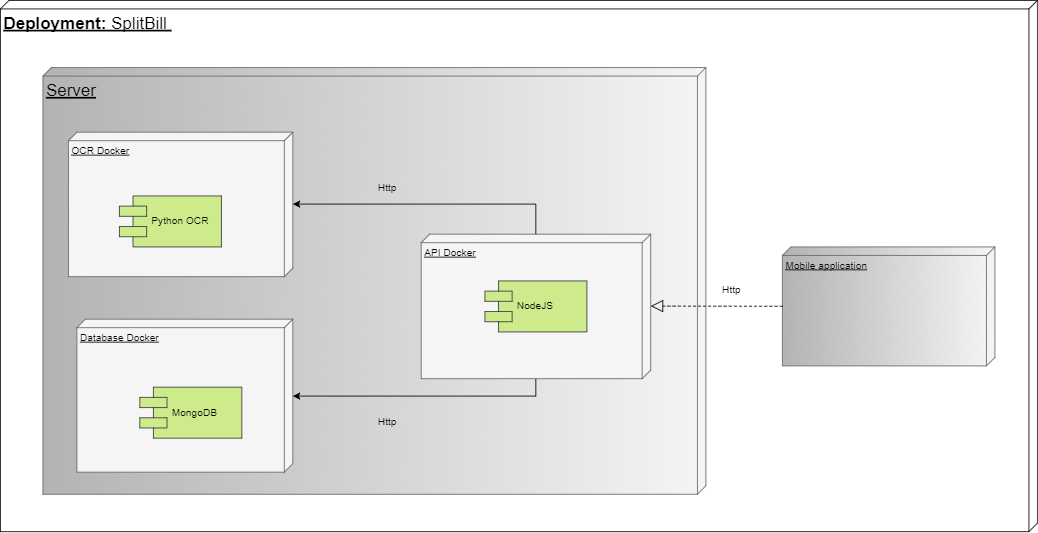
\includegraphics[width= \textwidth]{Deployment.png}
\caption{Deployment Diagram of the SplitBill system}
\centering
\end{figure}

\paragraph{Design patterns}
\subparagraph{} In this system the Gang of Four (GOF) observer pattern was used to ensure updates to the currently viewed bill is communicated to all devices while facilitating data hiding. There is a one to many relationship present where the API can communicate with multiple mobile devices, but the mobile devices can only communicate with the API and not any other devices with regards to the application. Updates to the bill on a single device have to be communicated to all active devices. The observer pattern ensures data hiding between all devices. When one mobile device makes changes to the currently active bill, the information is sent to the API, the observer, which is then responsible for communicating these changes to all mobile devices currently active on the bill. Applying the observer pattern ensures there is low coupling and separation of concerns. 

\subparagraph{} Another pattern used is the General Responsibility-Assignment Software Pattern (GRASP) the controller pattern. This pattern ensures that the user interfaces and business objects are independent and as such can change without affecting one another. The application installed on the mobile device is the user interface, this user interface does not handle any business tasks. All requests and changes initiated by the user interface are handled by the API, which means it serves as the controller. Having changes and requests sent to the API for processing before data is sent or retrieved from the OCR module or MongoDB database ensures that the user interface is independent of the business objects. This also allows multiple interfaces to be added without the need for major changes to support new interfaces. Having the controller pattern ensures there is design for change, high cohesion, low coupling and separation of concerns.   

       
    \subsection{Installation}
    The installation will be detailed as per module since modules can be swapped out for others with similar functionality if so required. 
    \subsubsection{API Module}
    \textbf{Initial requirements}
     	\begin{enumerate}
     	\item Ensure Docker is installed on the computer that will run the server. Get Docker here: \url{https://docs.docker.com/engine/installation/} 
        
        \item Note the IP address of this computer on the network so that Platypus-Mobile can be set to connect to it.
        
        \item Follow the instructions for Platypus-OCR in this document or  here: \url{https://github.com/COS301-brute-force/Platypus-OCR/wiki/Installation-Details} to set up the OCR component for this API to connect to.
     	\end{enumerate}
        
	\paragraph{Docker}
	The following commands must be run in order to get the API up and running on the server. Due to the nature of Docker, it will download all dependencies and run them. Please be patient.
    \vspace{1cm}
 
  \subparagraph{Environment:	source/default}  
    \subparagraph{}
	Build Docker:
    \begin{lstlisting}
		docker build -t cos301-brute-force/platypus-api:source-latest
	\end{lstlisting}
    
    \vspace{1cm}
    Run database:
    \begin{lstlisting}
    docker run \
  	-itd \
  	--rm \
  	--name platypus-db-source \
  	-p 27017 \
  	library/mongo:3.0.14
    \end{lstlisting}
    
    \vspace{1cm}
    
    Run API: 
     \begin{lstlisting}
	docker run \
	-it \
	--rm \
  	-e "NODE_ENV=source" \
  	-e "DEBUG=platypus-api*" \
  	--name platypus-api-source \
  	--link platypus-db-source \
  	-v /home/node/platypus-api/node_modules \
  	-v $(pwd):/home/node/platypus-api \
  	-p 3000:3000 \
  	-p 3002:3002 \
  	cos301-brute-force/platypus-api:source-latest
    \end{lstlisting}
    
    \vspace{1cm}
    
    Run tests: 
    \begin{lstlisting}
    docker run \
    -itd \
    --rm \
    -e "NODE_ENV=source" \
    -e "DEBUG=platypus-api*" \
    --name platypus-api-source \
    --link platypus-db-source \
    -v /home/node/platypus-api/node_modules \
    -v $(pwd):/home/node/platypus-api \
    -p 3000:3000 \
    -p 3002:3002 \
    cos301-brute-force/platypus-api:source-latest
    \end{lstlisting}
    
    \vspace{0.5cm}
 	\begin{lstlisting}
	docker exec -it platypus-api-source /bin/bash
	\end{lstlisting}
    
    \vspace{0.5cm}
 	\begin{lstlisting}
	docker run \
    -it \
    --rm \
    -e "NODE_ENV=source" \
    -e "DEBUG=platypus-api*" \
    --name platypus-api-source \
    --link platypus-db-source \
    -v /home/node/platypus-api/node_modules \
    -v $(pwd):/home/node/platypus-api \
    -p 3000:3000 \
    -p 3002:3002 \
    cos301-brute-force/platypus-api:source-latest npm test
    \end{lstlisting}
	
    \subparagraph{Environment:	dev}
    \subparagraph{}
     Build: 

	\begin{lstlisting}
	docker build -t cos301-brute-force/platypus-api:dev-latest
	\end{lstlisting}

	\vspace{1cm}
	Run database:

	\begin{lstlisting}
	docker run \
    -itd \
    --name platypus-db-dev \
    -p 27017 \
    library/mongo:3.0.14
	\end{lstlisting}
	
    \vspace{1cm}
	Run API:
	
	\begin{lstlisting}
	docker run \
  	-it \
  	--rm \
  	-e "NODE_ENV=development" \
  	-e "DEBUG=platypus-api*" \
  	--name platypus-api-dev \
  	--link platypus-db-dev \
  	-v /home/node/platypus-api/node_modules \
  	-v $(pwd):/home/node/platypus-api \
  	-p 3000:3000 \
  	-p 3002:3002 \
  	cos301-brute-force/platypus-api:dev-latest
	\end{lstlisting}
	
    \vspace{1cm}
	Run tests:

    \begin{lstlisting}
	docker run \
    -it \
    --rm \
    -e "NODE_ENV=development" \
    -e "DEBUG=platypus-api*" \
    --name platypus-api-dev \
    --link platypus-db-dev \
    -v /home/node/platypus-api/node_modules \
    -v $(pwd):/home/node/platypus-api \
    -p 3000:3000 \
    -p 3002:3002 \
    cos301-brute-force/platypus-api:dev-latest npm test
	\end{lstlisting}
	
    \vspace{1cm}
 
	\paragraph{Docker Swarm}
        This document gives step-wise instructions for building the docker swarm for the Platypus project as a whole.

	\subparagraph{Requirements}
	\subparagraph{}
	We are going to need multiple VMs to join together in a docker swarm. These
could be docker machines, KVM instances or physical nodes. For this
example, we will assume the following nodes:
\begin{itemize}
\item docker-swarm-manager-01 (192.168.3.30)
\item docker-swarm-manager-02 (192.168.3.31)
\item docker-swarm-manager-03 (192.168.3.32)
\item docker-swarm-worker-01 (192.168.3.33)
\item docker-swarm-worker-02 (192.168.3.34)
\item docker-swarm-worker-03 (192.168.3.35)
\item docker-swarm-worker-04 (192.168.3.36)
\end{itemize}

We need three managers, for redundancy and for consensus.

\subparagraph{Initialize}
\subparagraph{}
On the first docker-swarm-manager:
\vspace{0.5cm}
\begin{lstlisting}
docker swarm init
\end{lstlisting}
 \vspace{0.5cm}
You need to join nodes to the docker swarm, see  \url{https://docs.docker.com/engine/reference/commandline/swarm_join/} 
\vspace{0.5cm}
\begin{lstlisting}
docker service create \
  --name=swarm-visualizer-02 \
  -p 8080 \
  --constraint="node.role==manager" \
  --network platypus-private \
  --mount="src=/var/run/docker.sock,dst=/var/run/docker.sock,type=bind" \
  dockersamples/visualizer
\end{lstlisting}
\vspace{0.5cm}
\begin{lstlisting}
docker volume create platypus-db
docker volume create platypus-db-dev
\end{lstlisting}
\vspace{0.5cm}
\begin{lstlisting}
docker network create --driver=overlay platypus-private
docker network create --driver=overlay platypus-public
\end{lstlisting}
\vspace{0.5cm}
\begin{lstlisting}
docker service create \
  --name platypus-db-dev \
  --network platypus-private \
  --with-registry-auth \
  -p 27017 \
  --constraint 'node.hostname == docker-swarm-worker-04' \
  --mount "source=platypus-db-dev,target=/data/db,type=volume" \
  library/mongo:3.0.14
\end{lstlisting}
\vspace{0.5cm}
\begin{lstlisting}
docker service create \
  --name platypus-api-dev \
  -p 3000 \
  -e "NODE_ENV=development" \
  --network platypus-private \
  --with-registry-auth \
  compiax/platypus-api:dev-latest
\end{lstlisting}
\vspace{0.5cm}
\begin{lstlisting}
docker service create \
  --name platypus-ocr-dev \
  -p 5000:5000 \
  -e "FLASK_APP=server.py" \
  --network platypus-private \
  --with-registry-auth \
  compiax/platypus-ocr:dev-latest
\end{lstlisting}
\vspace{0.5cm}
\begin{lstlisting}
docker run \
  -it \
  --rm \
  -e "FLASK_APP=server.py" \
  --name platypus-ocr-source \
  -p 3001:5000 \
  cos301-brute-force/platypus-ocr:source-latest
\end{lstlisting}
\vspace{0.5cm}
\begin{lstlisting}
docker service create \
  --name students-proxy \
  -p 80:80 \
  -p 443:443 \
  --network odin-private \
  --network odin-public \
  --network platypus-private \
  --network platypus-public \
  --with-registry-auth \
  --replicas 2 \
  compiax/students-proxy
\end{lstlisting}

\subparagraph{Updating}
\subparagraph{}
\begin{lstlisting}
docker service update \
  --image compiax/platypus-api:dev-latest \
  --with-registry-auth \
  platypus-api-dev
\end{lstlisting}

\begin{lstlisting}
docker service update \
  --image compiax/students-proxy:latest \
  --with-registry-auth \
  students-proxy
\end{lstlisting}

\subparagraph{Useful Docker Service Commands}
\subparagraph{}

\begin{lstlisting}
docker service update \
  --publish-rm 8080 \
  --with-registry-auth \
  swarm-visualizer-01
\end{lstlisting}

\begin{lstlisting}
docker service update \
  --publish-rm 8080 \
  --with-registry-auth \
  swarm-visualizer-02
\end{lstlisting}

\begin{lstlisting}
docker service update \
  --publish-add 8080 \
  --with-registry-auth \
  swarm-visualizer-01
\end{lstlisting}

\begin{lstlisting}
docker service update \
  --publish-add 8080 \
  --with-registry-auth \
  swarm-visualizer-02
\end{lstlisting}

\begin{lstlisting}
docker service update \
  --publish-rm 3000 \
  --with-registry-auth \
  platypus-api-dev
\end{lstlisting}

\begin{lstlisting}
docker service update \
  --publish-add 3000 \
  --with-registry-auth \
  platypus-api-dev
\end{lstlisting}

\begin{lstlisting}
docker service update \
  --publish-rm 8000 \
  --with-registry-auth \
  platypus-daemon-dev
\end{lstlisting}

\begin{lstlisting}
docker service update \
  --publish-add 8000 \
  --with-registry-auth \
  platypus-daemon-dev
\end{lstlisting}


\subparagraph{SSL}
\subparagraph{}

\begin{lstlisting}
sudo openssl req -x509 -nodes -days 365 -newkey rsa:2048 -keyout ss.wildcard.split-bill.co.za.key -out ss.wildcard.split-bill.co.za.crt
\end{lstlisting}

\begin{lstlisting}
sudo openssl req -x509 -nodes -days 365 -newkey rsa:2048 -keyout ss.wildcard.wildcard.split-bill.co.za.
\end{lstlisting}

    \subsubsection{Mobile Module}
    Once SplitBill meets all user satisfaction criteria, it will be released on the Android store for public use. Currently, it is developed to run on \emph{Android KitKat (4.4)} or newer; however, SplitBill is envisioned and has the potential to be released on additional platforms such as Apple IOS. 
    
   \subparagraph{Initial requirements}
\begin{itemize}
\item Please ensure instructions to set up the API module have been followed accurately to ensure that the API is set up correctly.
\item Plug your \emph{Android} phone into your computer and enable developer options in the settings as explained here: 
\url {https://www.androidcentral.com/how-enable-developer-settings-android-42}
\end{itemize}



\subparagraph{Install}
\begin{enumerate}
\item Pull the dev branch of the Platypus-Mobile repository here: \url{ https://github.com/COS301-brute-force/Platypus-Mobile}
\item Install Ionic globally
	\begin{lstlisting}
		npm install -g cordova ionic
	\end{lstlisting}
\item Install the project dependencies
\begin{lstlisting}
		npm install
	\end{lstlisting}
\end{enumerate}

\subparagraph{Run}
\subparagraph{}
Run in browser
\begin{lstlisting}
		ionic serve
	\end{lstlisting}
   \vspace{1cm}
Run on mobile device setup for USB debugging
\begin{lstlisting}
		ionic cordova run android
	\end{lstlisting}
   \vspace{1cm}
Optional: Get application and server output in your Google Chrome browser
	\begin{lstlisting}
		chrome://inspect
	\end{lstlisting}

    \subsubsection{OCR Module}
       \subparagraph{Initial requirements}
Please ensure instructions to set up the API module have been followed accurately to ensure that the API is set up correctly.
    \subparagraph{Software overview:}
    \subparagraph{}
    
Software requirements include Python 2.7 and additional Python module PIL for image manipulation as well as OpenCV, Flask, Tesseract and its Python wrapper pytesseract. The following instructions include details for using our docker image for software installation.

\subparagraph{Docker}
\subparagraph{}
A Docker image can be used to support all the software required to run the module. Docker software details can be found at \url{https://www.docker.com/} under the Get Docker tab at the top of the page. There are installation details for various Operating Systems. Details of the docker image are as follows: 

Build:  
\vspace{0.5cm}
\begin{lstlisting}
docker build -t cos301-brute-force/platypus-ocr:source-latest
\end{lstlisting}
\vspace{0.5cm}

Run OCR:
\vspace{0.5cm}
\begin{lstlisting}
docker run \
  -it \
  --rm \
  -e "FLASK_APP=server.py" \
  --name platypus-ocr-source \
  -v $(pwd):/usr/src/app \
  -p 3001:5000 \
  cos301-brute-force/platypus-ocr:source-latest

\end{lstlisting}

    
\subsection{Getting started}
Ensure the latest version of the application is installed on your mobile phone and a server has been configured to handle requests from the SplitBill application. Ensure installation of all modules has been followed precisely according to the instructions provided in this document or on the various module's wiki entries: 
\begin{itemize}
\item \url{https://github.com/COS301-brute-force/Platypus-API/wiki/Installation}
\item \url{https://github.com/COS301-brute-force/Platypus-API/wiki/Docker-Swarm} 
\item \url{https://github.com/COS301-brute-force/Platypus-OCR/wiki/Installation} 
\item \url{https://github.com/COS301-brute-force/Platypus-Mobile/wiki/Installation}
\end{itemize}

Upon start-up of the application on the mobile device, the user will be prompted for a user-name which is not persisted to a database, and asked to choose a color to keep track of claimed items.
\subparagraph{}
The application's menus and pages and sufficiently self-explanatory when encountered for the first time. The application is designed to cater for all user groups who are familiar with an Android mobile device. 
\subparagraph{}
When creating a new bill your device's camera will open automatically. Make sure to capture the bill in good and even lighting to ensure the best results for the character recognition of the bill and its items.
\subparagraph{}
When you are happy with the quality of the picture, it will be uploaded to the server for processing with use of the optical character recognition module. This will produce a JSON string that is sent back to your device. Once the bill information is returned, your session is started and you will be presented with bill items. 
\subparagraph{}
You will be able to add additional users to the session. To do this, the other users should have the application installed on their devices and have network access. The initial user will use the menu item to navigate to the session code generated when the bill was uploaded. Additional users can now enter the code into the application on their own device. Once this has been done the system will retrieve the bill information and display it to the new users for use on their own devices. 
\subparagraph{}
In the bill information screen, you can swipe left on an item to open a menu in which you can claim single or multiple items. When items are claimed, the quantity of the items is reduced by the amount that you have claimed. Once the item’s amount has reached zero no user will be able to claim another instance of the item unless a user removes an instance from their own claimed items in the "My Items" menu. Swiping right on an item will open a menu in which you can edit the selected item's price, description or quantity. 
\subparagraph{}
At the bottom of the screen, you will see a running total due by you which includes a gratuity. Claiming an item adds the price of the item to the total. The gratuity has a default value of 10 percent of your current total amount but may be altered to be higher or lower. 
At the top right of a bill page is three horizontal lines which offer a menu when tapped. This contains menu items which should be self-explanatory and simplifies navigation. 
If you claimed an item by mistake and wish to remove it you should navigate to "My Items" in the menu or tap on "My Items" in the tab at the top of the page. Once there you may swipe left on the mistakenly claimed item and tapping the circle with a horizontal line through it will then delete the item from your claimed items.
\subparagraph{}
The final amount will be that of the prices of all the items you have claimed, and the amount of gratuity you wish to add. When the user is satisfied with the claimed items, gratuity, and final amount to pay, the user may leave the session. Leaving the session will clear the bill displayed on the device. Once the last person has left the session the session will be terminated. When this occurs, there is no way for the user to retrieve previous bill information.

\section{Using the system}
\subparagraph{Start-up: }
Upon start-up of the application the user is prompted for a nickname and a color. These values are stored locally. The user data is only stored in the server when a user joins or creates a session.  
\subparagraph{}
Once the user creates a session, a session ID is generated on the server and a new, empty Bill object is created. The bill is added to the database with the session ID. The user is then added to the session. The user is then prompted to take a picture of the bill. This image is then uploaded to the API via a POST request. The API sends the image to the OCR module via a POST request for processing. 
\subparagraph{Image processing and character recognition: }
The OCR module, as its name indicates, is responsible for optical character recognition of the bill image received from the API. The OCR module first enhances the received image in order to improve the quality of the character recognition output. It thresholds the image to obtain a gray-scale image, reduces noise and aligns the text using the OpenCV software. After character recognition has taken place using the Tesseract software, Levenshtein distance is used to calculate the difference between the word that the OCR recognized and words saved in a provided dictionary. When the distance is low enough, the word is replaced with the word found in the common dictionary.
\subparagraph{} The information of the bill is then extracted and irrelevant information such as items with empty descriptions, prices of zero or quantities of zero are removed from the JSON string and the remaining information is arranged in a JSON string before it is sent to the API. If the OCR is not able to recognize enough or any text the JSON string will contain error information that reflects this. 
\hspace{1cm}

If there was sensible text recognized from the image, the object will have the following format:

\begin{lstlisting}
{ "type": "success", "attributes": { "data":[ {"id":"1","desc":"description of item 1","price":"xx.xx","quantity":"1"}, {"id":"2","desc":"description of item 2","price":"xx.xx","quantity":"5"}, {"id":"3","desc":"description of item 3","price":"xx.xx","quantity":"3"} ] }, "relationships": { "data":{total":"xx.xx"} } }
\end{lstlisting}

\subparagraph{Displaying image information: }
When the API receives the information from the OCR module, it sends the information in a POST request back to the calling mobile application where the data is then displayed to the user along with the functionalities that accompany it. 
\subparagraph{Claiming an item: }
When the user swipes left on an item, the user is given the option to claim one, or multiple instances of the item. When an item or multiple items are claimed, the price corresponding to the items is added to the running total which can be seen at the bottom of the application screen. When an item is claimed, the quantity of the item available to claim is reduced by the amount that was claimed. When the quantity of an item reaches zero, users will no longer be able to claim items of this type unless a user removes a claim to the item or the item quantity is modified to a quantity larger than zero. 
\subparagraph{Editing an item: }
If the user swipes left on an item, they are presented with a menu in which they can alter the items price, description or quantity. This is useful for when the image was of inferior quality and character recognition was not 100\% accurate. 
\subparagraph{Adding an item: }
The user also has the option to add items to the current bill. An additional item will need a description, price and quantity and will be displayed to all active users. 
\subparagraph{Editing current claimed items: }
The “My Items” menu displays the items that the current user has already claimed. In this menu the user can swipe left on a selected item to increase or decrease the amount of the items claimed, or remove the item from their claimed items. Changes to quantities in this menu can also be observed in the main bill information screen and the running total for the user. 
\subparagraph{Observing the total and adjusting gratuity: }
At the bottom of the main screen, the total price of the claimed items along with a gratuity option is displayed. The gratuity has a default value of 10\% of your bill, but can be modified to be less or more, and is added to your running total accordingly.
\subparagraph{Adding users to the bill session: }
The application has the functionality to add additional users to the same bill session. When the bill session is started the session ID and bill information is stored in the database. An additional user can be added to the session by inputting the generated session ID into his/her own mobile device. When the session ID is sent to the API via a POST request, the API retrieves the bill information of the corresponding session ID stored in the database. The bill information is then sent to the mobile application for display and interaction. The API will now be responsible for the live communication of item changes between each device. As an item is either created, edited or claimed, the device performing the action emits the action to the API, which in turn emits the update to all connected devices.  
\subparagraph{Leaving a session: }
When the user is satisfied with their claimed items, gratuity and final total, the user can leave the session. Once a user selects the option to leave a session, the API is updated and removes the user from the session in the database. Once all users have left, the session is terminated. There is no persistent data storage for a session that has been concluded.


\section{Troubleshooting}	
   \subsection{API Module}
While the API is being run in development mode, there are debug messages that are output to the console. These messages are there to see what code is being called when, with details about the function call, data being passed, and generally what is currently happening.
\subparagraph{}
This allows the developer to monitor how the system is executing and be able to see exactly what is going on. This proved valuable feedback to assist in debugging and ensuring correct execution of the system.
	
    \subsection{Mobile Module}
 	\paragraph{Problem with the server?}
		Please see the API troubleshooting page
\paragraph{The application is not on your mobile device?}
\begin{itemize}
\item Ensure you ran the commands correctly as shown on the installation page
\item Check the application's directory on your mobile device since installing a new application doesn't necessarily make a shortcut on your home screen
\item Ensure your mobile device has developer settings switched on
\item Ensure your mobile device is plugged into the host issuing the installation commands
\end{itemize} 
\paragraph{The application doesn't open?}
\begin{itemize}
\item Ensure you're using an Android device 
\item Ensure your mobile device is version \emph{Android KitKat (4.4)} or newer
\end{itemize}

\paragraph{The interface is unusable or broken?}
Your solution may not be supported, please send a bug report to our team to fix this 
\paragraph{Creating a bill doesn't work or gives a timeout error?}
\begin{itemize}
\item Ensure you have SplitBill permission to use your camera when prompted upon launch. You may need to reinstall the application
\item Ensure you have an Internet connection or have some means of communicating with the server such as a LAN connection
\item Ensure the server didn't throw an error
\end{itemize}
    
    \subsection{OCR Module} 
     \paragraph{There is no text displayed?}
     If there is no text response after attempting to upload the bill picture, ensure the following: 
    \begin{itemize}
    \item Ensure you are connected to a network for communication with the server
    \item Ensure the server has been configured correctly and is running. See the installation details or troubleshooting for the API module.
    \end{itemize}
    \paragraph{Error message received after uploading an image?}
    When there is an error message, this means the character recognition failed. The Tesseract optical character recognition software is not yet perfect and may at times fail to recognize any meaningful characters or any characters at all. When this happens you can try to take a picture with that is closer up and has better lighting and alignment. 
    \paragraph{The text I am getting is not right? }
    If the information displayed to you is incorrect or absent, try taking a new photo that is closer up and has better lighting and alignment. The Tesseract recognition software is not perfect and thus will not yet be able to return exact character information each time. 
   
\end{document}
